\begin{figure}[h!]
    \centering
    \caption{Minimum wage levels in the US by jurisdiction, 2010--2019}
    \label{fig:mw_US}

    \begin{subfigure}{.7\textwidth}
        \caption{State policies}
        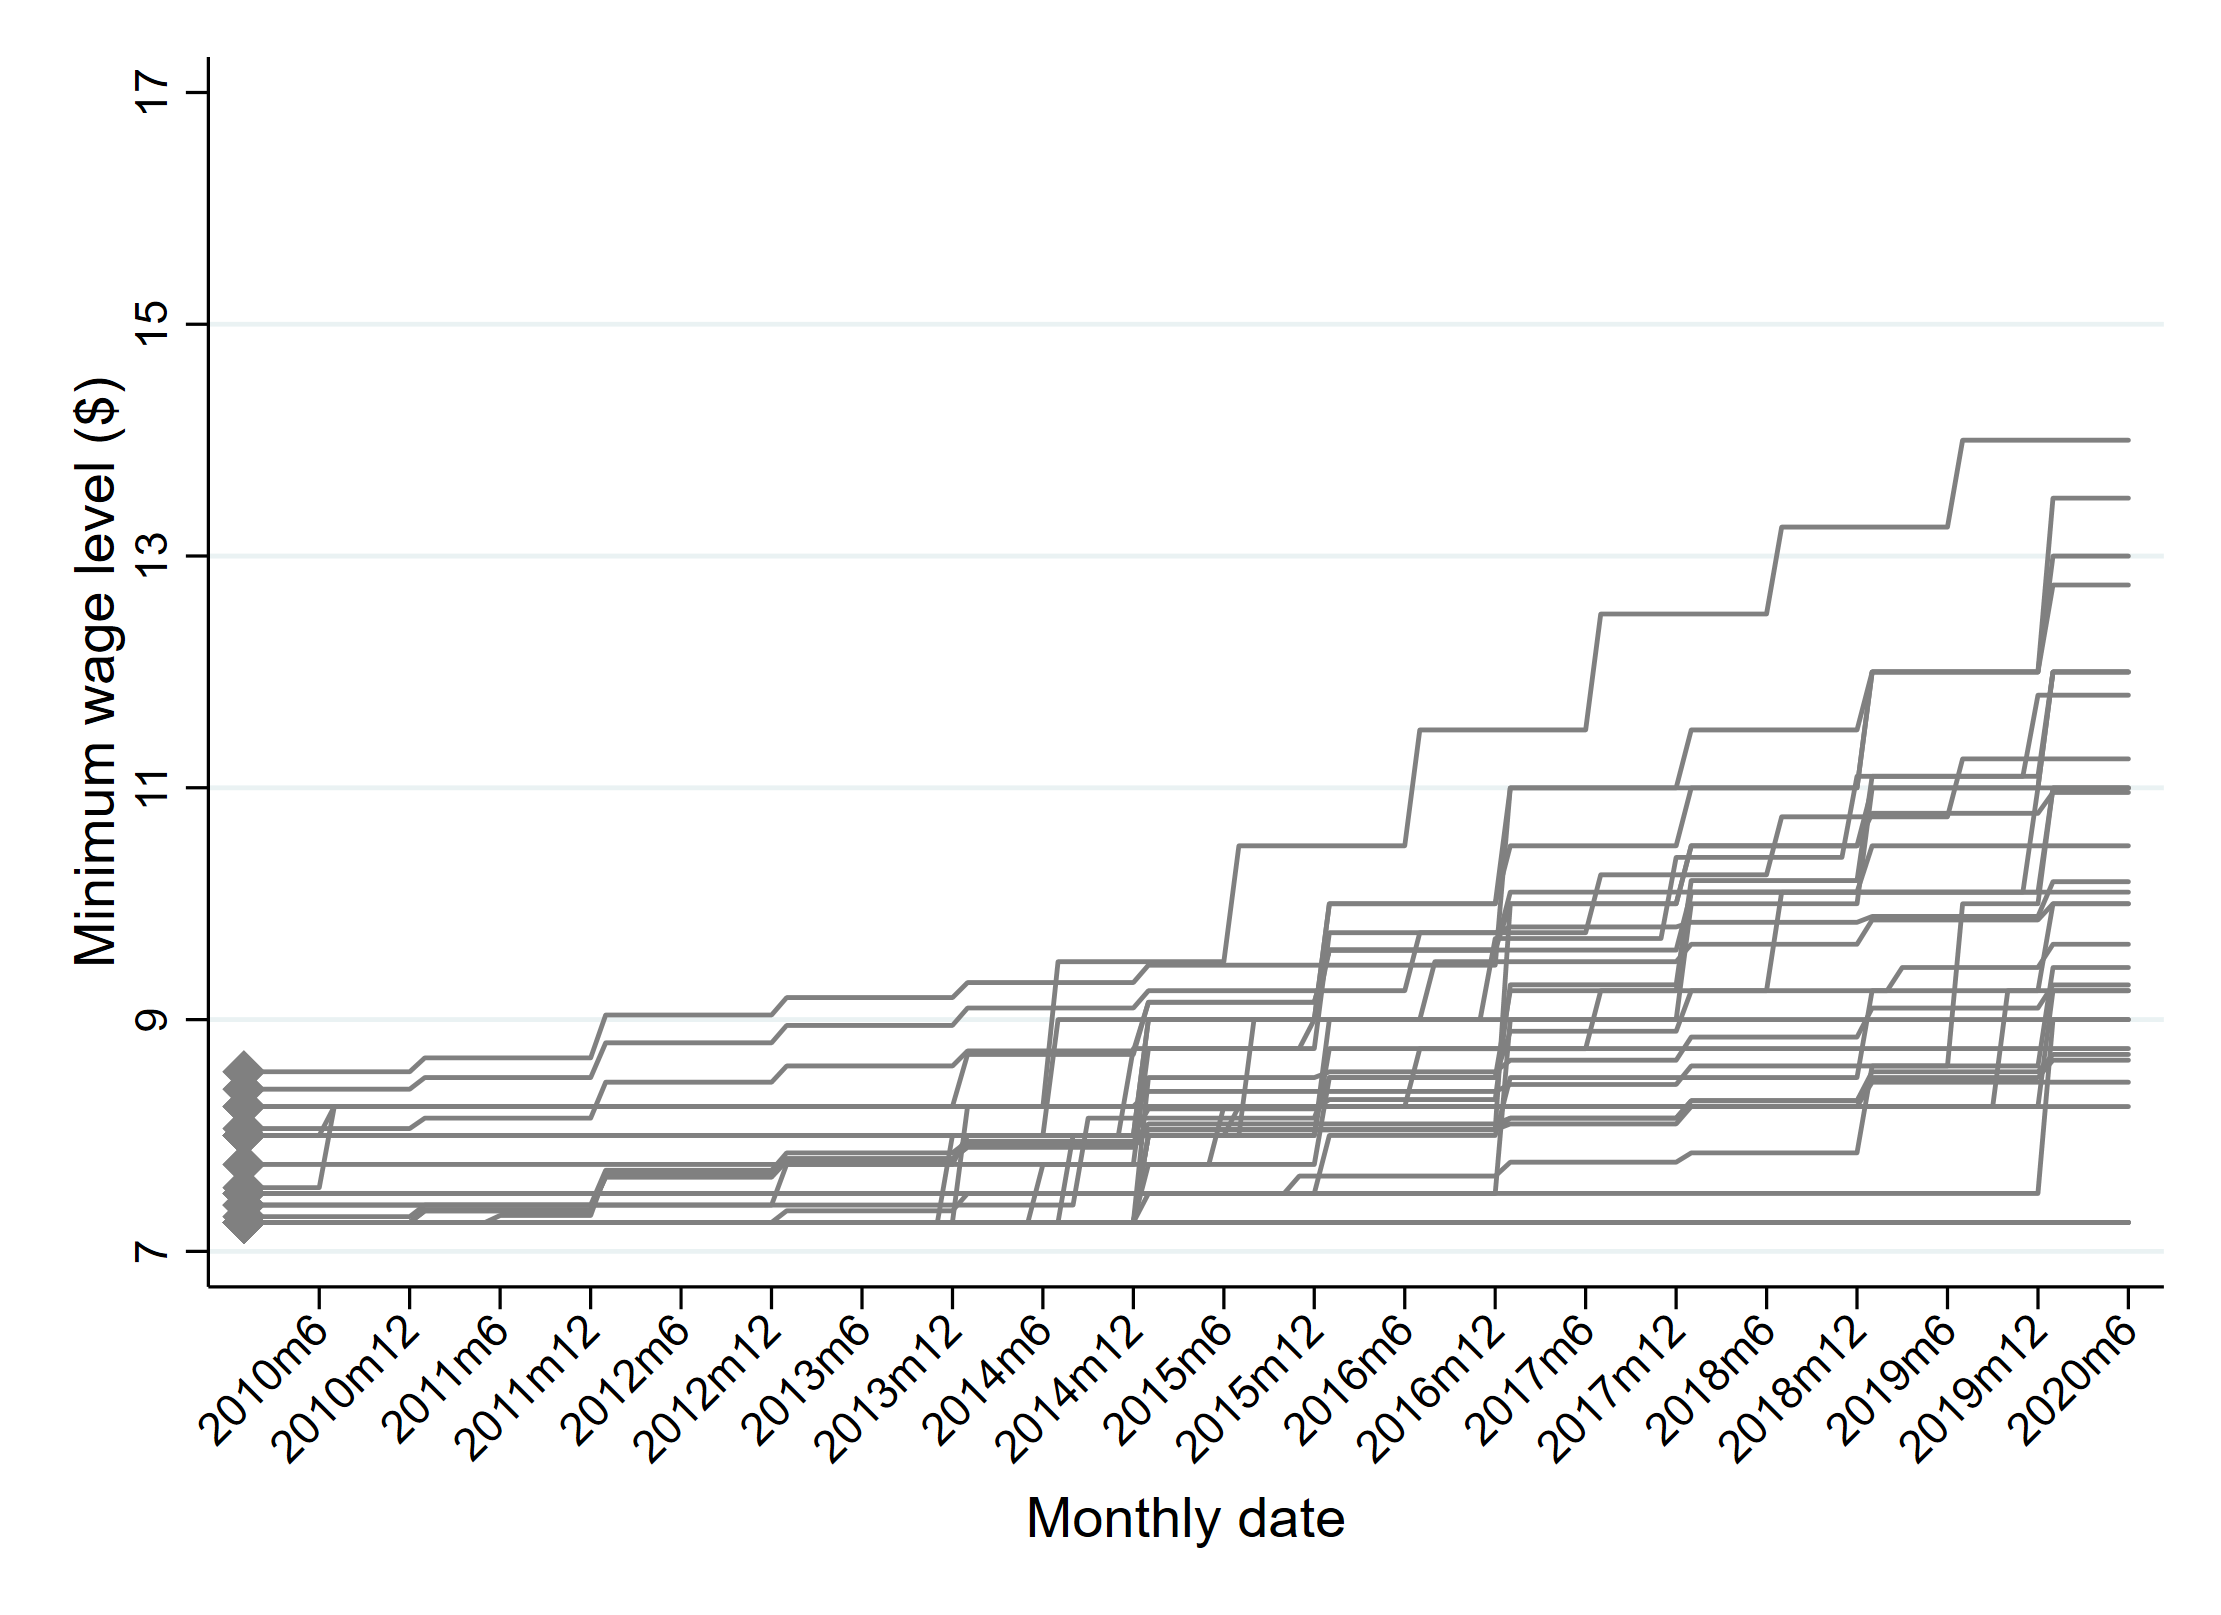
\includegraphics[width = \textwidth]
            {mw_US/output/state_mw_levels}
    \end{subfigure}\\
    \begin{subfigure}{.7\textwidth}
        \caption{Sub-state policies}
        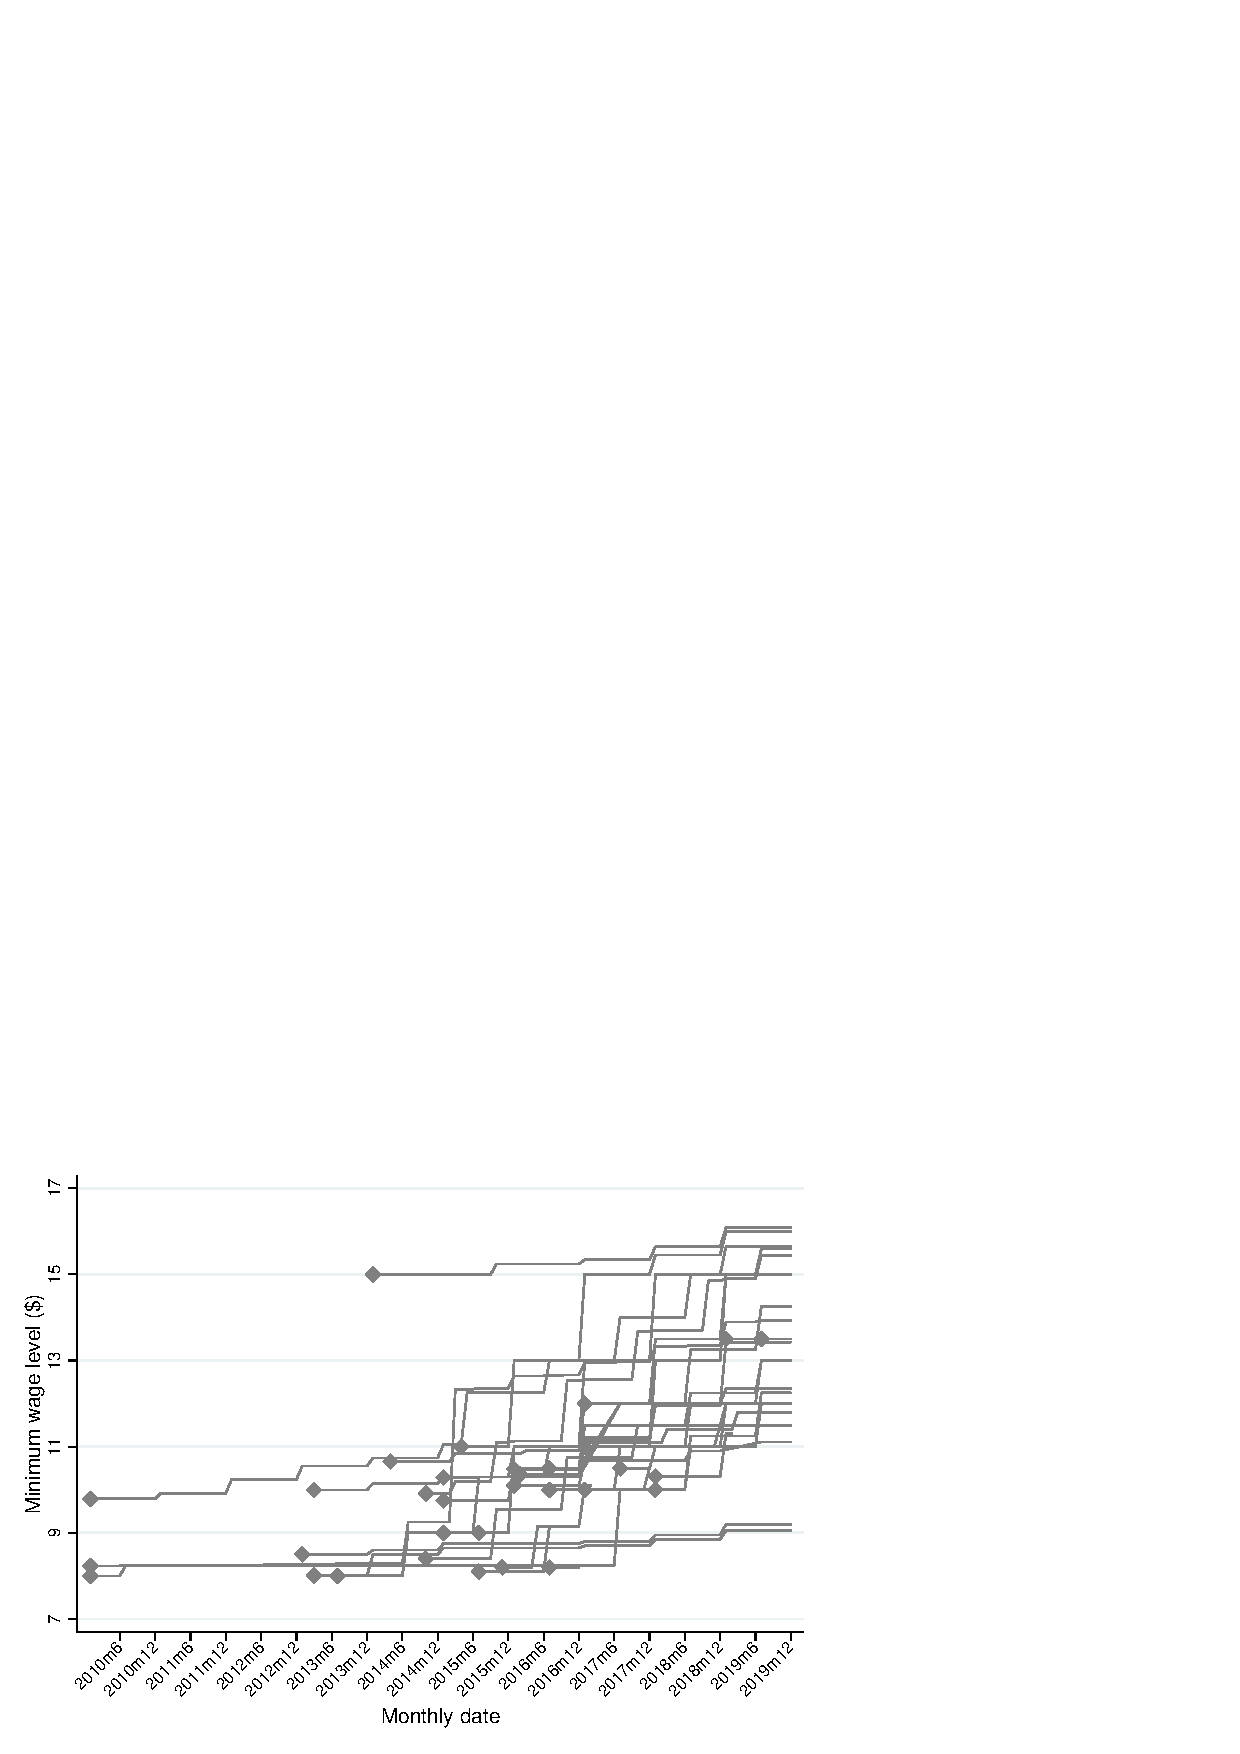
\includegraphics[width = \textwidth]
            {mw_US/output/local_mw_levels}
    \end{subfigure}

    \begin{minipage}{.95\textwidth} \footnotesize
        \vspace{3mm}
        Notes:
        Data are from the minimum wage panel described in 
        Section \ref{sec:mw_construction}.
        The plots show the levels of the minimum wage in the different 
        jurisdictions from January 2010 to December 2019.
        Panel (a) reports the state level policies.
        Panel (b) reports the sub-state level policies.
    \end{minipage}
\end{figure}
